% !TeX root = ../thesis.tex
% !TeX spellcheck = en_US

\chapter{Refactoring spreadsheets}
\label{chapter:implementingrefactorings}

\noindent
\begin{figure}[h!]
\hspace*{0.003\textwidth}
\begin{subfigure}[c]{0.1\textwidth}
\f{=1+2+3}
\end{subfigure}
\begin{subfigure}[c]{0.1\textwidth}
$\xrightarrow{Parsing}$
\end{subfigure}
\fbox{
\begin{subfigure}[c]{0.15\textwidth}
\begin{tikzpicture}[-latex ,auto ,node distance =1.3 cm and 0.5cm ,on grid , semithick,
,
state/.style ={ circle ,top color =white ,
draw, minimum width =0.75 cm}]
\node[state] (RootPlus) {$+$};
\node[state] (SecondPlus) [below right=of RootPlus] {$+$};
\node[state] (Input1) [below left=of RootPlus] {1};
\node[state] (Input2) [below left=of SecondPlus] {2};
\node[state] (Input3) [below right=of SecondPlus] {3};

\path (RootPlus) edge node {} (Input1);
\path (RootPlus) edge node {} (SecondPlus);
\path (SecondPlus) edge node {} (Input2);
\path (SecondPlus) edge node {} (Input3);
\end{tikzpicture}
\end{subfigure}
\begin{subfigure}[c]{0.14\textwidth}
$\xrightarrow{Refactoring}$
\end{subfigure}
\begin{subfigure}[c]{0.17\textwidth}
\begin{tikzpicture}[-latex ,auto ,node distance =1.3 cm and 0.5cm ,on grid , semithick,
,
state/.style ={ circle ,top color =white ,
draw, minimum width =0.75 cm}]
\node[state] (Root) {$F$};
\node[state] (11) [below left=of Root] {\tiny{\f{SUM}}};
\node[state] (12) [below right=of Root] {[]};
\node[state, node distance = 1.3cm and 0.85cm] (21) [below left =of 12] {1};
\node[state, node distance = 1.32cm and 0.85cm] (22) [below =of 12] {2};
\node[state, node distance = 1.3cm and 0.85cm] (23) [below right=of 12] {3};

\path (Root) edge node {} (11);
\path (Root) edge node {} (12);
\path (12) edge node {} (21);
\path (12) edge node {} (22);
\path (12) edge node {} (23);
\end{tikzpicture}
\end{subfigure}
}
\begin{subfigure}[c]{0.1\textwidth}
$\xrightarrow{Printing}$
\end{subfigure}
\begin{subfigure}[c]{0.145\textwidth}
\f{=SUM(1,2,3)}
\end{subfigure}
%\caption{This chapter details the AST to AST transformations that implement the refactorings.}
\caption{Overview of the refactoring process.}
\label{fig:chapterrefactoringintrofigure}
\end{figure}

Refactoring a spreadsheet involves changing the worksheets, cells and formulas in a workbook.
Excel provides an API to change the worksheet and cells, and most other elements of a workbook.
When it is desired to refactor formulas this means the original formula string must be changed into a new formula string.
This is usually implemented by parsing the formula, performing the desired transformations on the AST and then printing the AST back to a string form \cite{fowler1999refactoring}.
The inner workings of the parser are described in Chapter \ref{chapter:parsing}.
This chapter covers how the AST is transformed for each refactoring, as seen in Figure \ref{fig:chapterrefactoringintrofigure}.

The refactorings are implemented in the BumbleBee Excel Add-In\footnote{\url{http://spreadsheetlab.org/2015/10/12/bumblebee-an-excel-refactoring-add-in/}}, and presented to the user through a context menu as seen in Figure \ref{fig:contextmenu}.
This context-menu automatically determines if a refactoring can be performed on the specific selected cell(s) and disables inapplicable refactorings.

%Every section of this chapter describes a refactoring, except for the discussion section.
%Every section starts with the situations where the refactoring it is applicable, and how this is detected by BumbleBee.
%The following subsection details the user interface, followed by the implementation of the refactoring.
%If an earlier implementation exist, the section concludes with a description of the improvements.

\newpage

\section{\rf{Extract formula}}
\label{refac:extractformula}

The goal of the \rf{extract formula} refactoring is to move part of a formula expression, a sub-formula, to another cell, which has a number of potential use cases:

\begin{itemize}
\itemsep0em
\item Magic numbers or other constants can be extracted to a separate cell, thus making them easy to adjust.
\item A large or complicated formula can be made easier to understand by splitting it into more smaller components. This solves the \rf{Multiple Operations} smell \cite{hermans2014detecting}.
\item Reduce duplication in a formula by extracting common sub-formulas into another cell. This solves the \rf{Duplicated Formulas} smell \cite{hermans2014detecting}.
\end{itemize}

\subsection{User interface}

\begin{figure}
	\centering
	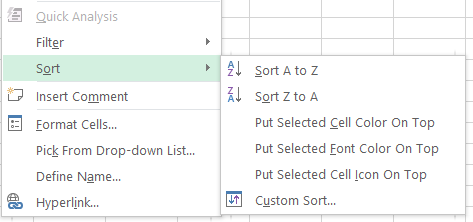
\includegraphics{implementation/contextmenu}
	\caption{BumbleBee context menu.}
	\label{fig:contextmenu}
\end{figure}

\begin{figure}
%\begin{minipage}[c][8cm][c]{0.5\textwidth}
%\centering
%\vspace*{\fill}
%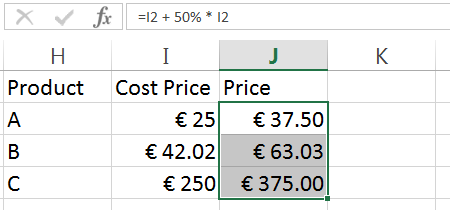
\includegraphics[height=3cm]{implementation/extractformula/21}
%\subcaption{User selects cells to be refactored}
%\label{fig:extractformulaexample2a}
%
%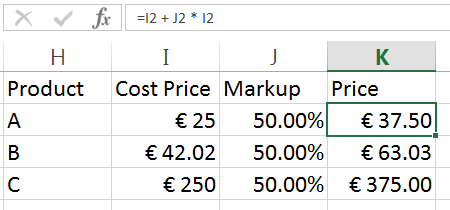
\includegraphics[height=3cm]{implementation/extractformula/23}
%\addtocounter{subfigure}{1}
%\subcaption{Refactoring has been performed}
%\label{fig:extractformulaexample2c}
%\end{minipage}
%\begin{minipage}[c][8cm][t]{0.5\textwidth}
%\vspace*{\fill}
%\centering
%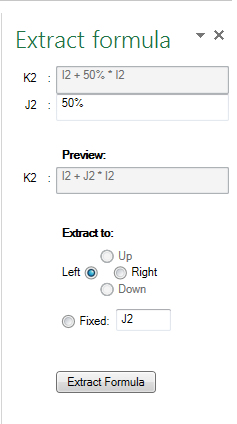
\includegraphics[height=7cm]{implementation/extractformula/22}
%\addtocounter{subfigure}{-2}
%\subcaption{User selects subformula to be extracted}
%\label{fig:extractformulaexample2b}
%\end{minipage}
\centering
\includegraphics{{implementation/extractformula/UI\string_Extractformula\string_arrows\string_pdf}}
\caption{An example application of \rf{Extract Formula}.}
\label{fig:extractformulaexample2}
\end{figure}

This refactoring requires the user to select cell(s) to be refactored, enter the subformula to be extracted and select where the extraction should occur to.
Figure \ref{fig:extractformulaexample2} shows the process as experienced by the user.
The user first selects the formulas to be extracted (Figure \ref{fig:extractformulaexample2}a) and clicks the Extract Formula entry in the refactoring context menu (not shown).
A side-panel pops out which allows the user to enter the sub-formula to be extracted and where it should be extracted to (Figure \ref{fig:extractformulaexample2}b) and presses the Extract Formula button.
In the example the \f{50\%} subformula was extracted to the left, and Figure \ref{fig:extractformulaexample2}c shows the situation after the user has named the new column.

\subsection{Implementation}

This subsection describes the details of the refactoring implementation, which consists of 2 parts: an AST tranformation of the formula, and a modification of the worksheet.
The first part operates solely on the formula and refactors it to the desired form, the second part handles actual placement of the formula in the cells and the moving if necessary.

\subsubsection{AST Transformation}
\label{subsec:astreplacementtransformation}

The AST transformation takes the original AST, the AST to replace and the replacement AST as inputs.
Then the original AST is traversed and every occurrence of the AST to replace is replaced by the replacement AST, yielding the new AST, this is illustrated in Figure \ref{fig:extractformulaASTtransformations}.
The C\# code for the AST replacement can be found in Listing \ref{lst:astreplace}.

This transformation is somewhat similar to the BumbleBee formula transformation rules.
However, it is complimentary rather than identical as can be seen by comparing Figure \ref{fig:extractformulaASTtransformations} and Figure \ref{fig:bbv1transformationrule}.
It might seem like the transformation rule "\f{=I2 + [a] * I2}" is suitable for this refactoring.
However, using transformation rules BumbleBee would have searched for the "outer" formula, keeping the \f{[a]} $\gets$ \f{50\%} available for the replacement rule.
In contrast, this transformation searches for the \f{[a]} "inner" formula, and replaces it with something different.

\subsubsection{Spreadsheet refactoring}

The AST replacement is performed on the original formula yielding a new formula, which is assigned to the cell that is being refactored.
If multiple cells are refactored at once, the AST replacement is performed on all of them.
Formulas with the same original R1C1 formula will have the same new R1C1 formula, so the AST replacement is only performed once per unique R1C1 formula and the resulting formula is re-used.

If the target of the extraction is a single cell, that cell gets assigned the subformula that will be extracted, otherwise if the user wants to extract in a direction, new cells are created in the appropriate direction and all will get assigned the subformula that will be extracted.

The C\# code for the spreadsheet refactoring can be found in Listing \ref{lst:extractformula}.

\begin{figure}
	\centering
	{
\begin{subfigure}[t]{0.12\textwidth}
\centering
\begin{tikzpicture}[-latex ,auto ,node distance =1.3 cm and 0.5cm ,on grid , semithick,
,
state/.style ={ circle ,top color =white ,
draw, minimum width =0.75 cm}]
\node[state] (Percent) {\tiny \%};
\node[state] (Constant50) [below =of Percent] {\tiny 50};

\path (Percent) edge node {} (Constant50);
\end{tikzpicture}
\caption*{${\scriptscriptstyle AST_{search}}$}
\end{subfigure}
}
{
\begin{subfigure}[t]{0.24\textwidth}
\centering
\begin{tikzpicture}[-latex ,auto ,node distance =1.3 cm and 0.8cm ,on grid , semithick,
,
state/.style ={ circle ,top color =white ,
draw, minimum width =0.75 cm}
,
redstate/.style ={ circle , fill=red,
draw, minimum width =0.75 cm}]
\node[state] (OpPlus) {$+$};
\node[state] (OpMult) [below right =of OpPlus] {$\ast$};

\node[state] (RefI2) [below left =of OpPlus] {\tiny Ref};
\node[state] (ConstI2) [below =of RefI2] {\tiny \f{I2}};

\path (RefI2) edge node {} (ConstI2);

\node[state] (RefI22) [below right = 1.3cm and 0.52cm of OpMult] {\tiny Ref};
\node[state] (ConstI22) [below =of RefI22] {\tiny \f{I2}};

\path (RefI22) edge node {} (ConstI22);

\node[redstate] (Percent) [below left = 1.3cm and 0.42cm of OpMult] {\tiny \%};
\node[redstate] (Constant50) [below =of Percent] {\tiny 50};

\path (Percent) edge node {} (Constant50);

\path (OpPlus) edge node {} (OpMult);
\path (OpPlus) edge node {} (RefI2);
\path (OpMult) edge node {} (RefI22);
\path (OpMult) edge node {} (Percent);
\end{tikzpicture}
\caption*{${\scriptscriptstyle AST_{or}}$}
\end{subfigure}
}
{
\begin{subfigure}[t]{0.12\textwidth}
\centering
\begin{tikzpicture}[-latex ,auto ,node distance =1.3 cm and 0.5cm ,on grid , semithick,
,
state/.style ={ circle ,top color =white ,
draw, minimum width =0.75 cm}]
\node[state] (RefJ2) {\tiny Ref};
\node[state] (ConstJ2) [below =of RefJ2] {\tiny \f{J2}};

\path (RefJ2) edge node {} (ConstJ2);
\end{tikzpicture}
\caption*{${\scriptscriptstyle AST_{repl}}$}
\end{subfigure}
}
{
\begin{subfigure}[b]{0.1\textwidth}
\centering
\vspace*{4em}
$\xrightarrow[Returns]{}$
\vspace*{2em}
\end{subfigure}
}
{
\begin{subfigure}[t]{0.24\textwidth}
\centering
\begin{tikzpicture}[-latex ,auto ,node distance =1.3 cm and 0.8cm ,on grid , semithick,
,
state/.style ={ circle ,top color =white ,
draw, minimum width =0.75 cm}
,
greenstate/.style ={ circle , fill=green,
draw, minimum width =0.75 cm}]
\node[state] (OpPlus) {$+$};
\node[state] (OpMult) [below right =of OpPlus] {$\ast$};

\node[state] (RefI2) [below left =of OpPlus] {\tiny Ref};
\node[state] (ConstI2) [below =of RefI2] {\tiny \f{I2}};

\path (RefI2) edge node {} (ConstI2);

\node[state] (RefI22) [below right = 1.3cm and 0.52cm of OpMult] {\tiny Ref};
\node[state] (ConstI22) [below =of RefI22] {\tiny \f{I2}};

\path (RefI22) edge node {} (ConstI22);

\node[greenstate] (RefJ2) [below left = 1.3cm and 0.42cm of OpMult] {\tiny Ref};
\node[greenstate] (ConstJ2) [below =of RefJ2] {\tiny \f{J2}};

\path (RefJ2) edge node {} (ConstJ2);

\path (OpPlus) edge node {} (OpMult);
\path (OpPlus) edge node {} (RefI2);
\path (OpMult) edge node {} (RefI22);
\path (OpMult) edge node {} (Percent);
\end{tikzpicture}
\caption*{${\scriptscriptstyle AST_{new}}$}
\end{subfigure}
}
	\caption{AST transformation to implement extract formula refactoring}
	\label{fig:extractformulaASTtransformations}
\end{figure}

\begin{figure}
	\centering
	{
\begin{subfigure}[t]{0.12\textwidth}
\centering
\tiny\f{I2 + [a] * I2}
\caption*{{\tiny Origin rule}}
\end{subfigure}
}
{
\begin{subfigure}[t]{0.24\textwidth}
\centering
\begin{tikzpicture}[-latex ,auto ,node distance =1.3 cm and 0.8cm ,on grid , semithick,
,
state/.style ={ circle ,top color =white ,
draw, minimum width =0.75 cm}
,
redstate/.style ={ circle , fill=red,
draw, minimum width =0.75 cm}]
\node[redstate] (OpPlus) {$+$};
\node[redstate] (OpMult) [below right =of OpPlus] {$\ast$};

\node[redstate] (RefI2) [below left =of OpPlus] {\tiny Ref};
\node[redstate] (ConstI2) [below =of RefI2] {\tiny \f{I2}};

\path (RefI2) edge node {} (ConstI2);

\node[redstate] (RefI22) [below right = 1.3cm and 0.52cm of OpMult] {\tiny Ref};
\node[redstate] (ConstI22) [below =of RefI22] {\tiny \f{I2}};

\path (RefI22) edge node {} (ConstI22);

\node[state] (Percent) [below left = 1.3cm and 0.42cm of OpMult] {\tiny \%};
\node[state] (Constant50) [below =of Percent] {\tiny 50};

\path (Percent) edge node {} (Constant50);

\path (OpPlus) edge node {} (OpMult);
\path (OpPlus) edge node {} (RefI2);
\path (OpMult) edge node {} (RefI22);
\path (OpMult) edge node {} (Percent);
\end{tikzpicture}
\caption*{{\tiny Matching AST}}
\end{subfigure}
}
{
\begin{subfigure}[t]{0.14\textwidth}
\centering
\tiny\f{\ldots\ [a] \ldots}
\caption*{{\tiny Target rule}}
\end{subfigure}
}
{
\begin{subfigure}[b]{0.1\textwidth}
\centering
\vspace*{4em}
$\xrightarrow[Returns]{}$
\vspace*{2em}
\end{subfigure}
}
{
\begin{subfigure}[t]{0.24\textwidth}
	\centering
	\begin{tikzpicture}[-latex ,auto ,node distance =1.3 cm and 1.0cm ,on grid , semithick,
	,
	state/.style ={ circle ,top color =white ,
		draw, minimum width =0.75 cm}
	,
	redstate/.style ={ circle , fill=red,
		draw, minimum width =0.75 cm}
	,
	greenstate/.style ={ circle , fill=green,
		draw, minimum width =0.75 cm}]
	\node[greenstate] (OpPlus) {\tiny\ldots};
	\node[greenstate] (OpMult) [below right =of OpPlus] {\tiny\ldots};
	
	\node[greenstate] (RefI2) [below left =of OpPlus] {\tiny\ldots};
	
	%\node[state] (Percent) [below left = 1.3cm and 0.42cm of OpMult] {\tiny \%};
	\node[state] (Percent) [below = of OpPlus] {\tiny \%};
	\node[state] (Constant50) [below =of Percent] {\tiny 50};
	
	\path (Percent) edge node {} (Constant50);
	
	\path (OpPlus) edge node {} (OpMult);
	\path (OpPlus) edge node {} (RefI2);
	\path (OpPlus) edge node {} (Percent);
	\end{tikzpicture}
	\caption*{{\tiny New AST}}
\end{subfigure}
}
	\caption{BumbleBee transformation rule}
	\label{fig:bbv1transformationrule}
\end{figure}

\newpage

\subsection{Detection of applicability}

\rf{Extract formula} is always applicable to a formula cell, as even a very simple formula like \f{=A1} still has a component that can be extracted.
In this case if \f{=A1} would be extracted to \f{B1} the original cell would become \f{=B1}.
This could be repeated endlessly, similar to how one could always extract a method that only consists of a call to another method.
Whether it is a good thing to perform this refactoring is dubious, but BumbleBee relies on the user to make this assessment.

\subsection{Improvements over RefBook's \rf{Extract row or column} and \rf{Extract Literal}}
\label{subsubsec:improvementsextractformula}

Two specialized versions of this refactoring were previously described by Bamade and Dig \cite{badame2012refactoring} and implemented in their RefBook tool.
RefBook's \rf{Extract Row or column} and \rf{Extract Literal} refactorings can both be performed by \rf{Extract formula}.
We have chosen to not keep the \rf{extract row or column} refactoring name because it does not fully describe the refactoring (a full row or column does not necessarily have to be extracted) and to keep the name in line with refactoring names in other domains.

The RefBook \rf{extract literal} refactoring can put a constant value into a cell and replace the occurrences of it with references to that cell, which can also be achieved with the BumbleBee \rf{extract formula} refactoring.
In addition this is possible for any constant expression, an expression without references, instead of only for constants.

The BumbleBee \rf{Extract Formula} refactoring has several advantages over Badame's implementation of \rf{Extract row or column}.
Firstly RefBook does not handle operator precedence.
This can be very problematic for this refactoring, because one of the most important properties of a refactoring should be that it does not change the program results.
Note that the RefBook authors were aware of this deficiency, and left this as future work.
This future work has been performed by the thesis author.

Secondly RefBook can only handle a single row or column, which must have exactly the same R1C1 formula in every cell.
It can only extract the subformula to a column to the right of the original range or a row above the original range.
BumbleBee can handle arbitrarily shaped ranges, with the only requirement that the subformula to be extracted occurs in all selected cells.
Furthermore in addition to extracting to a cell neighboring the original formula cell (up, down, left or right) it can also extract the subformula to a single shared cell location, which is very useful to remove duplication.

\section{\rf{Inline Formula}}
\label{refac:inlineformula}

The goal of the \rf{Inline Formula} refactoring is to replace all references to a cell with its contents and delete the original cell, and is therefore the inverse of the \rf{Extract Formula} refactoring.
For example if \f{A1} would contain \f{=1+1} and \f{B1} contains \f{=A1*2}, after applying this refactoring to \f{A1} \f{B2} would contain \f{=(1+1)*2}. 
The main potential use case for this formula is when the contents of a cell are clearer or just as clear as a cell reference.
It can also be used to solve the \rf{Long Calculation Chain} smell \cite{hermans2014detecting}.

While single cell references (e.g. \f{=SUM(A1,A2,A3)}) can always be inlined, a cell referenced as part of a range (e.g. \f{=SUM(A1:A3)}) can not always be inlined.
If in the previous example \f{A1} would contain \f{20}, the first formula would turn out fine: \f{=SUM(20,A2,A3)}, while the formula \f{=SUM(20:A3)} is invalid.
It might be possible to handle inlining into ranges using array formulas, but the extra complexity this would introduce in the formulas never outweighs the benefit of inlining in the authors opinion.
Some formulas might be able to be rewritten, e.g. \f{=SUM(A1:A3)} could become \f{=SUM(20,A2:A3)}, but this does not work in every case (e.g. \f{A1} cannot be inlined into \f{=A1:A5 3:3}) and thus such behavior has a higher chance to introduce errors and confuse users.
For these reasons the implementation does not perform the refactoring if the cell is referenced as part of a range.

For similar reasons, this refactoring cannot be performed on cells which are part of a named range consisting of more than one cell.

\subsection{User interface}

The refactoring is a one-click refactoring that is activated from the cell context menu, no additional user input is normally needed.

If one of the selected cells is referenced as part of a range, the user gets the choice to either abort the refactoring or continue replacing all references where the cell isn't part of a range.

\begin{figure}
	\centering
	{
\begin{subfigure}[t]{0.12\textwidth}
\centering
\begin{tikzpicture}[-latex ,auto ,node distance =1.3 cm and 0.5cm ,on grid , semithick,
,
state/.style ={ circle ,top color =white ,
	draw, minimum width =0.75 cm}]
\node[state] (RefJ2) {\tiny Ref};
\node[state] (ConstJ2) [below =of RefJ2] {\tiny \f{J2}};

\path (RefJ2) edge node {} (ConstJ2);
\end{tikzpicture}
\caption*{{\tiny AST to replace}}
\end{subfigure}
}
{
\begin{subfigure}[t]{0.24\textwidth}
\centering
\begin{tikzpicture}[-latex ,auto ,node distance =1.3 cm and 0.8cm ,on grid , semithick,
,
state/.style ={ circle ,top color =white ,
	draw, minimum width =0.75 cm}
,
redstate/.style ={ circle , fill=red,
	draw, minimum width =0.75 cm}
,
greenstate/.style ={ circle , fill=green,
	draw, minimum width =0.75 cm}]
\node[state] (OpPlus) {$+$};
\node[state] (OpMult) [below right =of OpPlus] {$\ast$};

\node[state] (RefI2) [below left =of OpPlus] {\tiny Ref};
\node[state] (ConstI2) [below =of RefI2] {\tiny \f{I2}};

\path (RefI2) edge node {} (ConstI2);

\node[state] (RefI22) [below right = 1.3cm and 0.52cm of OpMult] {\tiny Ref};
\node[state] (ConstI22) [below =of RefI22] {\tiny \f{I2}};

\path (RefI22) edge node {} (ConstI22);

\node[redstate] (RefJ2) [below left = 1.3cm and 0.42cm of OpMult] {\tiny Ref};
\node[redstate] (ConstJ2) [below =of RefJ2] {\tiny \f{J2}};

\path (RefJ2) edge node {} (ConstJ2);

\path (OpPlus) edge node {} (OpMult);
\path (OpPlus) edge node {} (RefI2);
\path (OpMult) edge node {} (RefI22);
\path (OpMult) edge node {} (RefJ2);
\end{tikzpicture}
\caption*{{\tiny Original AST}}
\end{subfigure}
}
{
\begin{subfigure}[t]{0.14\textwidth}
\centering
\begin{tikzpicture}[-latex ,auto ,node distance =1.3 cm and 0.5cm ,on grid , semithick,
,
state/.style ={ circle ,top color =white ,
	draw, minimum width =0.75 cm}]
\node[state] (Percent) {\tiny \%};
\node[state] (Constant50) [below =of Percent] {\tiny 50};

\path (Percent) edge node {} (Constant50);
\end{tikzpicture}
\caption*{{\tiny Replacement AST}}
\end{subfigure}
}
{
\begin{subfigure}[b]{0.1\textwidth}
\centering
\vspace*{4em}
$\xrightarrow[Returns]{}$
\vspace*{2em}
\end{subfigure}
}
{
\begin{subfigure}[t]{0.24\textwidth}
\centering
\begin{tikzpicture}[-latex ,auto ,node distance =1.3 cm and 0.8cm ,on grid , semithick,
,
state/.style ={ circle ,top color =white ,
	draw, minimum width =0.75 cm}
,
redstate/.style ={ circle , fill=red,
	draw, minimum width =0.75 cm}
,
greenstate/.style ={ circle , fill=green,
	draw, minimum width =0.75 cm}]
\node[state] (OpPlus) {$+$};
\node[state] (OpMult) [below right =of OpPlus] {$\ast$};

\node[state] (RefI2) [below left =of OpPlus] {\tiny Ref};
\node[state] (ConstI2) [below =of RefI2] {\tiny \f{I2}};

\path (RefI2) edge node {} (ConstI2);

\node[state] (RefI22) [below right = 1.3cm and 0.52cm of OpMult] {\tiny Ref};
\node[state] (ConstI22) [below =of RefI22] {\tiny \f{I2}};

\path (RefI22) edge node {} (ConstI22);

\node[greenstate] (Percent) [below left = 1.3cm and 0.42cm of OpMult] {\tiny \%};
\node[greenstate] (Constant50) [below =of Percent] {\tiny 50};

\path (Percent) edge node {} (Constant50);

\path (OpPlus) edge node {} (OpMult);
\path (OpPlus) edge node {} (RefI2);
\path (OpMult) edge node {} (RefI22);
\path (OpMult) edge node {} (Percent);
\end{tikzpicture}
\caption*{{\tiny New AST}}
\end{subfigure}
}
	\caption{The AST transformation for \rf{Inline Formula}, which is the inverse of the \rf{Extract Formula} transformation in Figure \ref{fig:extractformulaASTtransformations}.}
	\label{fig:inlineformulaAST}
\end{figure}

\newpage

\subsection{Implementation}
\label{subsec:inlineformulaimplementation}

If a formula cell $D$ contains a reference to cell $P$, $D$ is called a dependent of $P$, and $P$ is called a precedent of $D$.
This refactoring works by first collecting all dependents of the to be inlined cell.
This information is provided by Excel, although it could be manually constructed by parsing all formulas and building a dependency graph.

In every dependent a reference to the to be inlined cell is replaced by its contents, using the same AST transformation used by \rf{Extract Formula} as described in Section \ref{subsec:astreplacementtransformation}, with a reference to the cell as the AST to replace and the cell contents as the replacement AST.
This is also illustrated in Figure \ref{fig:inlineformulaAST}, which shows the \rf{Inline Formula} inverse action of the transformation performed in Figure \ref{fig:extractformulaASTtransformations}.
If the refactoring is successful, the original cell is deleted.

The refactoring can be performed on multiple cells at the same time.
To achieve this the above process is simply repeated.

The C\# code for this spreadsheet refactoring can be found in Listing \ref{lst:inlineformula}.

\subsection{Detection of applicability}

As described in the introduction of this section, \rf{Inline Formula} is applicable to all cells which have dependents but are not referenced as part of ranges.
For speed purposed however, the BumbleBee refactoring context menu only check whether the cell has any dependents.
Doing the full check would introduce significant delay every time the user would right click.

\newpage

\section{\rf{Introduce Cell Name}}
\label{refac:introducecellname}

As noted in Chapter \ref{chapter:anatomy}, a cell or range can have a user defined name.
If the user has defined a name for a cell or range, this name can be used in formulas instead of its location.

This is the motivation for the \rf{Introduce Cell Name} refactoring which was defined by Badame and Dig \cite{badame2012refactoring}.
With this refactoring, a user can define a name for a cell, and all references to that cell will be replaced the name.

BumbleBee re-implements this refactoring, with as an additional functionality to name a range of cells and replace all references to that range with the name.

\subsection{User Interface}

Excel has a ``Define Name'' option in cell the context-menu, but it lacks the functionality to also perform this refactoring.
The refactoring context-menu for this option closely mirrors the Excel user interface, and is called ``Define and Use Name''.
After the user clicks it, he enters a new name in a dialog box and the refactoring is performed.

\subsection{Implementation}

This implementation also uses the notion of dependents and precedence, which is explained in Section \ref{subsec:inlineformulaimplementation}.

First the cell or range is given the name supplied by the user.
Then in every dependent a reference to the now named cell is replaced by its name, using the same AST transformation used by \rf{Extract Formula} as described in Section \ref{subsec:astreplacementtransformation}.

The C\# code for this spreadsheet refactoring can be found in Listing \ref{lst:introducecellname}.

\subsection{Detection of applicability}

This refactoring shares the detection of applicability with \rf{Inline Formula}: if the cell or range is referenced anywhere in the spreadsheet 

\subsection{Improvements over RefBook's \rf{Introduce Cell Name}}

BumbleBee's version incorporates a small improvements over RefBook's refactoring: it not only works on cells, but also on ranges.

\newpage

\section{\rf{Group References}}
\label{refac:groupreferences}

In the spreadsheet formula language, some built-in functions have the ability to accept a variable number of arguments, most prominently \f{SUM}, the most commonly used function \cite{hermans2015enron}.
These functions also accept ranges, and thus the formulas \f{=SUM(A1,A2,A3,A4)} and \f{=SUM(A1:A4)} are equivalent.
The \rf{Group References} refactoring assumes spreadsheet users prefer the latter, and merges multiple adjacent cell references into a single range reference.
The refactoring can be used to solve the \rf{Multiple References} \cite{hermans2014detecting} smell if the referenced cells are adjacent but referred to separately.
The refactoring was defined but not implemented by Hermans et. al \cite{hermans2014detecting}

\subsection{User Interface}

The refactoring is a one-click refactoring that is activated from the cell context menu, no additional user input is needed.

\subsection{Implementation}

\subsubsection{Grouping algorithm}

In order to find the best grouping we have to solve the following problem: given a sheet with a certain set of cells selected, what are the ranges that select exactly those cells and do so with a minimum amount of ranges?

It turns out that this is a NP-hard problem, because it has a straightforward translation to a NP-hard version of the Polygon Covering problem \cite{masek1979some}, specifically covering a rectilinear polygon (the selected cells) with axis-parallel rectangles (ranges), allowing for holes.
This allows us to use an approximation algorithm or heuristic.
A $O(\sqrt{\log{n}})$ approximation algorithm for this specific problem has been found by Kumar and Ramesh \cite{kumar2003covering}, but implementing this would take a non-trivial amount of effort.

However, rather than implementing a heuristic ourselves, this is currently delegated to Excel which contains this functionality.
The algorithm Excel uses for this is unknown.

\subsubsection{Spreadsheet Refactoring}

The implementation traverses the formula AST, and, for every function with a variable number of arguments it encounters, groups its references by excluding all non-references (e.g. constants) and sending these to Excel to be grouped.
The function arguments then are replaced by grouped references and the AST is printed back to the formula cell.
References are processed separately depending on their absolute markers, e.g. \f{A1},\f{\$A1}, \f{A\$1} and \f{\$A\$1}, because grouping references with different markers cannot be done without changing the meaning of the formula.

\noindent If multiple cells are selected, the refactoring is repeated for every one.

\noindent The C\# code for this refactoring can be found in Listing \ref{lst:groupreferences}

\subsection{Detection of applicability}

This refactoring will be available to the user if the formula contains two or more references.

\section{\rf{Introduce Aggregate}}
\label{refac:introduceaggregate}

In the spreadsheet formula language, three binary operators have an equivalent aggregate function that accepts any number of arguments: \f{+} corresponds to \f{SUM}, \f{*} to \f{PRODUCT} and \f{\&} to \f{CONCATENATE}.

Thus a formula like \f{=A1+A2+A3+A4} can be rewritten to \f{=SUM(A1,A2,A3,A4)}, which is what the \rf{Replace Awkward Formula} refactoring, defined by Badame and Dig \cite{badame2012refactoring}, does.
The refactoring is especially useful when combined with the \rf{group references} refactoring, which rewrites it to \f{=SUM(A1:A4)}.

The author proposes an alternate name for this refactoring, \rf{Introduce Aggregate}, for two reasons.
Firstly \rf{Replace Awkward Formula} does not describe very good what the refactoring does, as more types of ``Awkward Formulas'' could be thought of which cannot be handled.
For example a formula with multiple nested \f{IF}s like \f{=IF(IF(IF(\ldots),FALSE,TRUE),A1,B1)} could be described as ``awkward'', but this refactoring does not replace it.
Secondly this keeps the name consistent with the \rf{Introduce Conditional Aggregate} refactoring.

\subsection{User Interface}

This refactoring is a one-click refactoring that is activated from the cell context menu, no additional user input is needed.
In the user interface it will always transparently be followed by the \rf{Group References} refactoring.

The refactoring shares a menu item with \nameref{refac:introduceconditionalaggregate}, as the operator will be changed to a SUMIF if applicable.
The menu item is called ``Change to SUM or SUMIF'' to make it easier to understand for users, because \rf{Introduce (Conditional) Aggregate} is abstract and contains jargon.
While ``Change to SUM or SUMIF'' does not fully describe the refactoring, this will be the most common use case and easy to understand for spreadsheet users.

\subsection{Implementation}

The implementation traverses the formula AST until it encounters the first operator it can refactor.
The left subtree then gets added to a list of arguments for the aggregate function, and the right subtree gets checked to see if it corresponds to the same operator.
If it is, the process gets repeated until a non-operator right subtree is encountered, at which point that subtree is the final addition to the argument list.
Note that this works because all operators are left-associative in Excel.
If operator has other associativities the algorithm would have to be slightly altered.

The C\# code for this refactoring can be found in listing \ref{lst:introduceaggregate}.

\subsection{Detecting applicability}

This refactoring will only be offered to the user if the top layer of a formula cell consisting of one of the applicable operators (\f{+},\f{*} or \f{\&})

\newpage

\subsection{Improvements over RefBook's \rf{Replace Awkward Formula}}

The concept of the \rf{Introduce Aggregate}/\rf{Replace Awkward Formula} refactoring is not complicated, and therefore not many improvements can be made.
However, BumbleBee does improve over RefBook in several ways related to this refactoring.

A first improvement in BumbleBee's implementation comes through the underlying parser: the RefBooks parser does not take operator precedence into account, and therefore a formula like \f{=1 + 2 * 3 + 4} would be refactored into \f{=SUM(1,2 * 3 + 4)} by RefBook, while BumbleBee refactors it into \f{=SUM(1,2 * 3,4)}.

A second improvement comes by combining this refactoring with two other refactorings through the user interface.
Combining this refactoring with \rf{Group References} allows a formula like \f{=A1+A2+A3+A4} to be rewritten into \f{=SUM(A1:A4)} instead of just \f{=SUM(A1,A2,A3,A4)}.
Combining this refactoring with \rf{Introduce Conditional Aggregate} when the spreadsheet data allows for this enables a formula like \f{=B12+B24+B36} to be rewritten into \f{=SUMIF("2015", B:B)} instead of just \f{=SUM(B12,B24,B36)}.

\clearpage

\section{\rf{Introduce Conditional Aggregate}}
\label{refac:introduceconditionalaggregate}

\begin{figure}
	\centering
	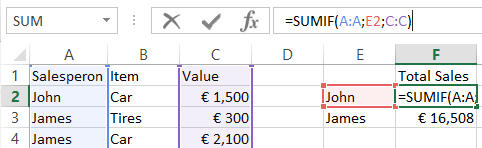
\includegraphics{implementation/aggregate/sumifexample}
	\caption{An example spreadsheet which uses \f{SUMIF}.}
	\label{fig:sumifexample}
\end{figure}

\begin{figure}
	\centering
	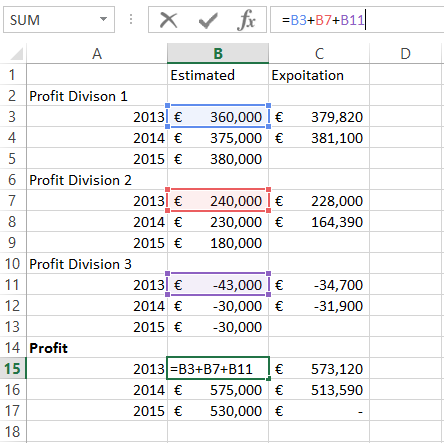
\includegraphics{implementation/aggregate/condaggrexample}
	\caption{An example where \f{SUMIF} could be used, but is not.}
	\label{fig:sumifcouldbeused}
\end{figure}

Three aggregate functions also have conditional counterparts: \f{SUMIF}, \f{AVERAGEIF} and \f{COUNTIF}.
These functions take two mandatory arguments: \textbf{check_range}, \textbf{condition} and the optional \textbf{operating_range}.
If \textbf{operating_range} is absent it equals \textbf{check_range}, with \f{COUNTIF} not supporting \textbf{operating_range} at all.
These functions evaluate the \textbf{condition} on every cell of \textbf{operating_range}, and if it is met the function's operation is performed on the corresponding cell from \textbf{operating_range}.

Examples make this clearer: \f{=SUMIF(A:A, "> 10")} sums all cells in column \f{A} that contain a value larger than \f{10}, and \f{=SUMIF(A:A, E2, C:C)} sums the cell from column \f{C} of every row where the cell value from column \f{A} equals \f{E2} , as illustrated in Figure \ref{fig:sumifexample}.

The conditional aggregate functions are powerful tools, but they are not always used. 
Instead what we often encountered is the ``Manual'' selection of the correct cells and summing these, as illustrated in Figure \ref{fig:sumifcouldbeused}.
When combining this refactoring with the \rf{Introduce Aggregate} refactoring we can rewrite \f{=B3+B7+B11} to \f{=SUM(B3,B7,B11)}, and that to \f{=SUMIF(A:A, "2015", B:B)}.
Because this was the most common pattern we will focus on \f{SUM} and \f{SUMIF}, but the refactoring works identical for \f{COUNT} to \f{COUNTIF} and \f{AVERAGE} to \f{AVERAGEIF}.

\subsection{User Interface}

This refactoring shares a context menu entry with \rf{Introduce Aggregate}.

\subsection{Implementation}

In order to see if a \f{SUM} can be rewritten to a \f{SUMIF}, we must determine if there is another range of cells with a value that uniquely identifies the summed cells.
In relational database theory, this is a concept known as a \emph{functional dependency}.
Several algorithms exist to automatically find functional dependencies, such as Dep-Miner \cite{lopes2000efficient}, FUN \cite{novelli2001fun} and TANE \cite{huhtala1999tane}, where FUN has been applied in a spreadsheet context \cite{cunha2009spreadsheets}.

Due to implementation time constraints, these algorithms were not used, and instead only a very simple but useful scenario is supported: the summed values are in a single row or column, and there is a single row or column that has a single unique value in it which can serve as the condition for \f{SUMIF}.
Figure \ref{fig:introcondaggrScenario1} shows such a scenario: column \f{A} uniquely determines the summed values and the formula can thus be rewritten to \f{=SUMIF(A:A, "A", B:B)}.
Figure \ref{fig:introcondaggrScenario2} shows a case where this is not possible: \f{A4} differs from \f{A1} and \f{A2} meaning there is no column that determines the summed values.
Figure \ref{fig:introcondaggrScenario2} shows another impossible case: here column \f{A} determines the summed values, but there is an additional row with an identical value in cell \f{A5} and thus column \f{A} does not \emph{uniquely} determine the summed values.
Additionally, the refactoring is not supported if the summed cells are not in a single row or column.

The C\# code that performs the refactoring if the above conditions are met can be found in Listing \ref{lst:introduceconditionalaggregate}.

\begin{figure}
	\centering
	\begin{subfigure}[t]{0.25\textwidth}
		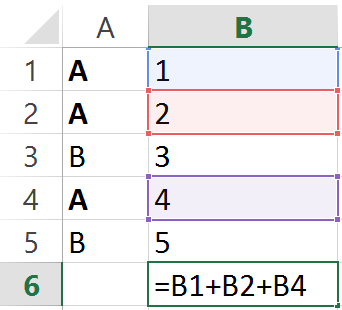
\includegraphics[width=\textwidth]{implementation/aggregate/scenario1}
		\caption{Supported: \newline Column \f{A} uniquely determines which values are summed.}
		\label{fig:introcondaggrScenario1}
	\end{subfigure}
	\hspace{0.05\textwidth}
	\begin{subfigure}[t]{0.25\textwidth}
		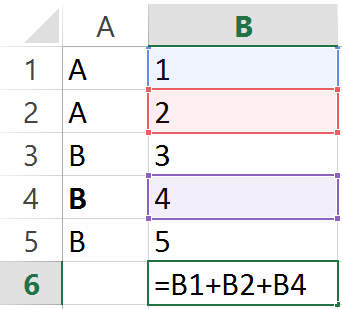
\includegraphics[width=\textwidth]{implementation/aggregate/scenario2}
		\caption{Unsupported: \newline No column determines which values are summed.}
		\label{fig:introcondaggrScenario2}
	\end{subfigure}
	\hspace{0.05\textwidth}
	\begin{subfigure}[t]{0.25\textwidth}
		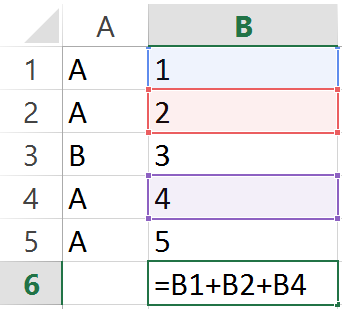
\includegraphics[width=\textwidth]{implementation/aggregate/scenario3}
		\caption{Unsupported: \newline Column \f{A} does not determine which values are summed, because \f{B5} is not summed.}
		\label{fig:introcondaggrScenario3}
	\end{subfigure}
	\caption{Example scenarios of \rf{Introduce Conditional Aggregate}}
	\label{fig:introcondaggrScenario}
\end{figure}

\subsection{Detection of applicability}

This refactoring is activated only as part of the \rf{Introduce Aggregate} refactoring, and therefore shares its detection of applicability.
Any further detection is performed within the code that implements the refactoring itself.

%\section{\rf{Fixate References}}
%
%\todo{Unsure of ik deze nog wil implementeren, maar lijkt zeer laaghangend fruit.}
%
%The Fixate References is similar to the \rf{Make Cell Constant} refactoring described by Badame \cite{badame2012refactoring}.
%Maar beter want: user kan zelf selecteren welke cellen wel/niet absolute.
%
%"Fixate references" beschrijft 100x beter wat de refactoring doet dan "Make cell constant". "Make cell constant" zou eerder impliceren dat je het resultaat van de cell berekening neemt en dat opslaat i.p.v. de formula. Wat trouwens ook weer een potentiele refactoring is, maar misschien een beetje een anti-pattern in excel.
%

\newpage

\section{Discussion}

\subsection{Undo and redo functionality}

It must be noted that all refactorings have a major deficiency: they cannot be undone with the Excel undo function.
This is not a limitation inherent to the refactorings, the previous state could be remembered and some refactorings even have a well-defined inverse refactoring.

The reason that undo and redo functionality is not available in BumbleBee is a technical limitation imposed by Excel: the Excel undo-redo stack is not available to Excel Add-Ins.
Instead, as soon as a Excel Add-In changes the Excel spreadsheet file, in fact as soon as it interacts with the internal document model even if it does not change anything, the Excel undo-redo stack gets cleared.
In an industrial-strength application this functionality would be essential.

A workaround is possible by manually maintaining an undo stack, however this was deemed outside of the scope of this thesis.
This workaround also does not integrate well with Excel and does not allow changes made outside of the Add-In to be undone. 
As long as Excel keeps this restriction this will always be a severe limitation to any tool that automatically changes spreadsheet files for the user.

\subsection{Future improvement possibilities}

\rf{Extract formula} could benefit from more UI support.
If the user could select the formula to be extracted from within the Excel formula editor the user interface could be streamlined.
Another possibility would be to determine candidate subformulas that the user could extract, and present these in a list.
Generating a list of all subformulas is fairly trivial, but this list can become very large, especially in the longer formulas that would benefit from this refactoring.
A heuristic which can prune the list of subformulas could improve this experience.

A minor deficiency in the current \rf{Extract Formula} code is that is does not fully handle the commutative operators \f{+} and \f{*}.
An operator is commutative if the order of the operands does not matter: \f{1 + 2} is equal to \f{2 + 1}.
BumbleBee's equality comparer takes this into account, and tries the reverse order of the operands for \f{+} and \f{*} if it does not find a match.
However, this does not fully solve the problem: the formula \f{=1 + 2 + 3} is parsed as \f{=(1 + 2) + 3}, thus if the user wishes to extract \f{2 + 3} BumbleBee will report an error since it does not encounter \f{2 + 3} in the AST.

The \rf{Introduce Conditional Aggregate} automated refactoring currently only supports a very basic scenario.
The algorithm only checks if a single column determines another column, and furthermore the algorithm is not proven correct.
Both of these problems could be solved by properly determining functional dependencies using an established algorithm.
Functional dependencies where two or more columns determine the content of a single column can be supported through the \f{SUMIFS}, \f{AVERAGEIFS} and \f{COUNTIFS} functions. For example \f{=SUMIFS(C:C,A:A,2015,B:B,"John")} sums the values from column \f{C} of the rows where column \f{A} contains \f{2015} and column \f{B} contains \f{"John"}, which corresponds to column \f{C} being dependent on columns \f{A} and \f{B}.